\section{Results}
\label{sec:results}

\subsection{Case Study 1: Transform Comparison}
\label{sec:results_transforms}

Table~\ref{tab:transforms} summarizes the performance of all six 1D-to-2D spectral transformations evaluated with EfficientNet-B0 on the GreenHyperSpectra dataset. The direct Reshape transformation achieved the highest mean $R^2$ of 0.684 $\pm$ 0.001 across eight plant traits, representing a substantial improvement of +0.097 over the supervised EfficientNet-1D baseline reported by \citet{cherif2025greenhyperspectra} ($R^2 = 0.587$). Reshape also exhibited the lowest variance across random seeds, indicating robust and reproducible performance. The continuous wavelet transform (CWT, $R^2 = 0.641 \pm 0.004$) and multi-window spectrogram ($R^2 = 0.636 \pm 0.025$) ranked second and third, respectively, though with notably higher inter-seed variability in the case of the spectrogram. The two-dimensional correlation spectroscopy (2D-COS, $R^2 = 0.625$) and Gramian Angular Fields (GAF, $R^2 = 0.623$) yielded moderate improvements over the 1D baseline, while the Markov Transition Field (MTF, $R^2 = 0.426$) was the only transformation that performed substantially worse than the 1D approach.

Five of six transformations surpassed the 1D-CNN baseline, demonstrating that the conversion of hyperspectral signals to two-dimensional image representations captures spectral information that one-dimensional convolutional architectures fail to exploit. The consistent superiority of the simpler Reshape transformation over more computationally intensive methods such as CWT and 2D-COS suggests that preserving the sequential ordering of wavelengths---where spatially adjacent pixels correspond to spectrally proximate bands---provides sufficient spatial structure for 2D convolutions to learn inter-band relationships.

\begin{table}[htbp]
\centering
\caption{Comparison of 1D-to-2D spectral transformations for multi-trait retrieval using EfficientNet-B0 on the GreenHyperSpectra dataset. Mean $R^2$ and standard deviation are reported across three random seeds (155, 240, 318). All methods are compared against the supervised EfficientNet-1D baseline of \citet{cherif2025greenhyperspectra} ($R^2 = 0.587$). The best result per column is shown in bold.}
\label{tab:transforms}
\begin{tabular}{llccr}
\toprule
Transform & Channels & Mean $R^2$ $\pm$ std & $\Delta$ vs.\ 1D & Seeds \\
\midrule
\textbf{Reshape}     & 1 & \textbf{0.684 $\pm$ 0.001} & \textbf{+0.097} & 3 \\
CWT                   & 1 & 0.641 $\pm$ 0.004          & +0.054          & 3 \\
Spectrogram           & 3 & 0.636 $\pm$ 0.025          & +0.049          & 3 \\
2D-COS                & 2 & 0.625                      & +0.038          & 1 \\
GAF                   & 2 & 0.623                      & +0.036          & 1 \\
MTF                   & 1 & 0.426                      & $-$0.161        & 1 \\
\midrule
Cherif 1D-CNN         & -- & 0.587                     & --              & 3 \\
\bottomrule
\end{tabular}
\end{table}


\subsection{Per-Trait Analysis}
\label{sec:results_per_trait}

Table~\ref{tab:per_trait} presents the per-trait comparison between the best 2D method (Reshape) and the 1D baseline. The 2D approach improved retrieval accuracy for all eight traits, with improvements ranging from +0.008 for protein content (C\textsubscript{p}) to +0.245 for carbon-based constituents (C\textsubscript{bc}). The largest gains were observed for traits related to leaf structural composition: C\textsubscript{bc} ($\Delta R^2 = +0.245$), anthocyanins ($\Delta R^2 = +0.174$), and leaf mass per area ($\Delta R^2 = +0.122$). These traits are characterised by broad, overlapping absorption features across multiple spectral regions, suggesting that the 2D representation enables the model to capture cross-band correlations that are informative for their retrieval. Pigment-related traits (chlorophyll, carotenoids) showed moderate improvements (+0.070 to +0.080), while canopy-level traits (LAI, +0.041; equivalent water thickness, +0.036) and protein content (+0.008) exhibited smaller but consistent gains.

\begin{table}[htbp]
\centering
\caption{Per-trait $R^2$ comparison between the best 2D method (Reshape + EfficientNet-B0) and the supervised 1D baseline \citep{cherif2025greenhyperspectra}. Values for the 2D method are averaged across three random seeds; values for Cherif are from their reported results. The best value per trait is shown in bold.}
\label{tab:per_trait}
\begin{tabular}{lccr}
\toprule
Trait & Cherif 1D & Reshape 2D & $\Delta$ \\
\midrule
C\textsubscript{ab} (Chlorophyll)    & 0.517 & \textbf{0.597} & +0.080 \\
C\textsubscript{ar} (Carotenoids)    & 0.621 & \textbf{0.691} & +0.070 \\
C\textsubscript{anth} (Anthocyanins) & 0.454 & \textbf{0.628} & +0.174 \\
C\textsubscript{w} (EWT)             & 0.667 & \textbf{0.703} & +0.036 \\
C\textsubscript{m} (LMA)             & 0.651 & \textbf{0.773} & +0.122 \\
LAI                                   & 0.563 & \textbf{0.604} & +0.041 \\
C\textsubscript{p} (Protein)         & 0.679 & \textbf{0.687} & +0.008 \\
C\textsubscript{bc} (CBC)            & 0.544 & \textbf{0.789} & +0.245 \\
\midrule
\textbf{Mean}                         & 0.587 & \textbf{0.684} & \textbf{+0.097} \\
\bottomrule
\end{tabular}
\end{table}


Figure~\ref{fig:scatterplot} shows observed versus predicted values for all eight traits using the best model configuration (Reshape + EfficientNet-B0). Strong agreement along the 1:1 line is evident for leaf mass per area ($R^2 = 0.773$), carbon-based constituents ($R^2 = 0.787$), and carotenoids ($R^2 = 0.707$). Chlorophyll content ($R^2 = 0.570$) and leaf area index ($R^2 = 0.592$) show greater scatter, particularly at higher observed values, reflecting the inherent difficulty of these retrievals from canopy-level reflectance where saturation effects are well documented \citep{cherif2025greenhyperspectra}.

\begin{figure}[htbp]
    \centering
    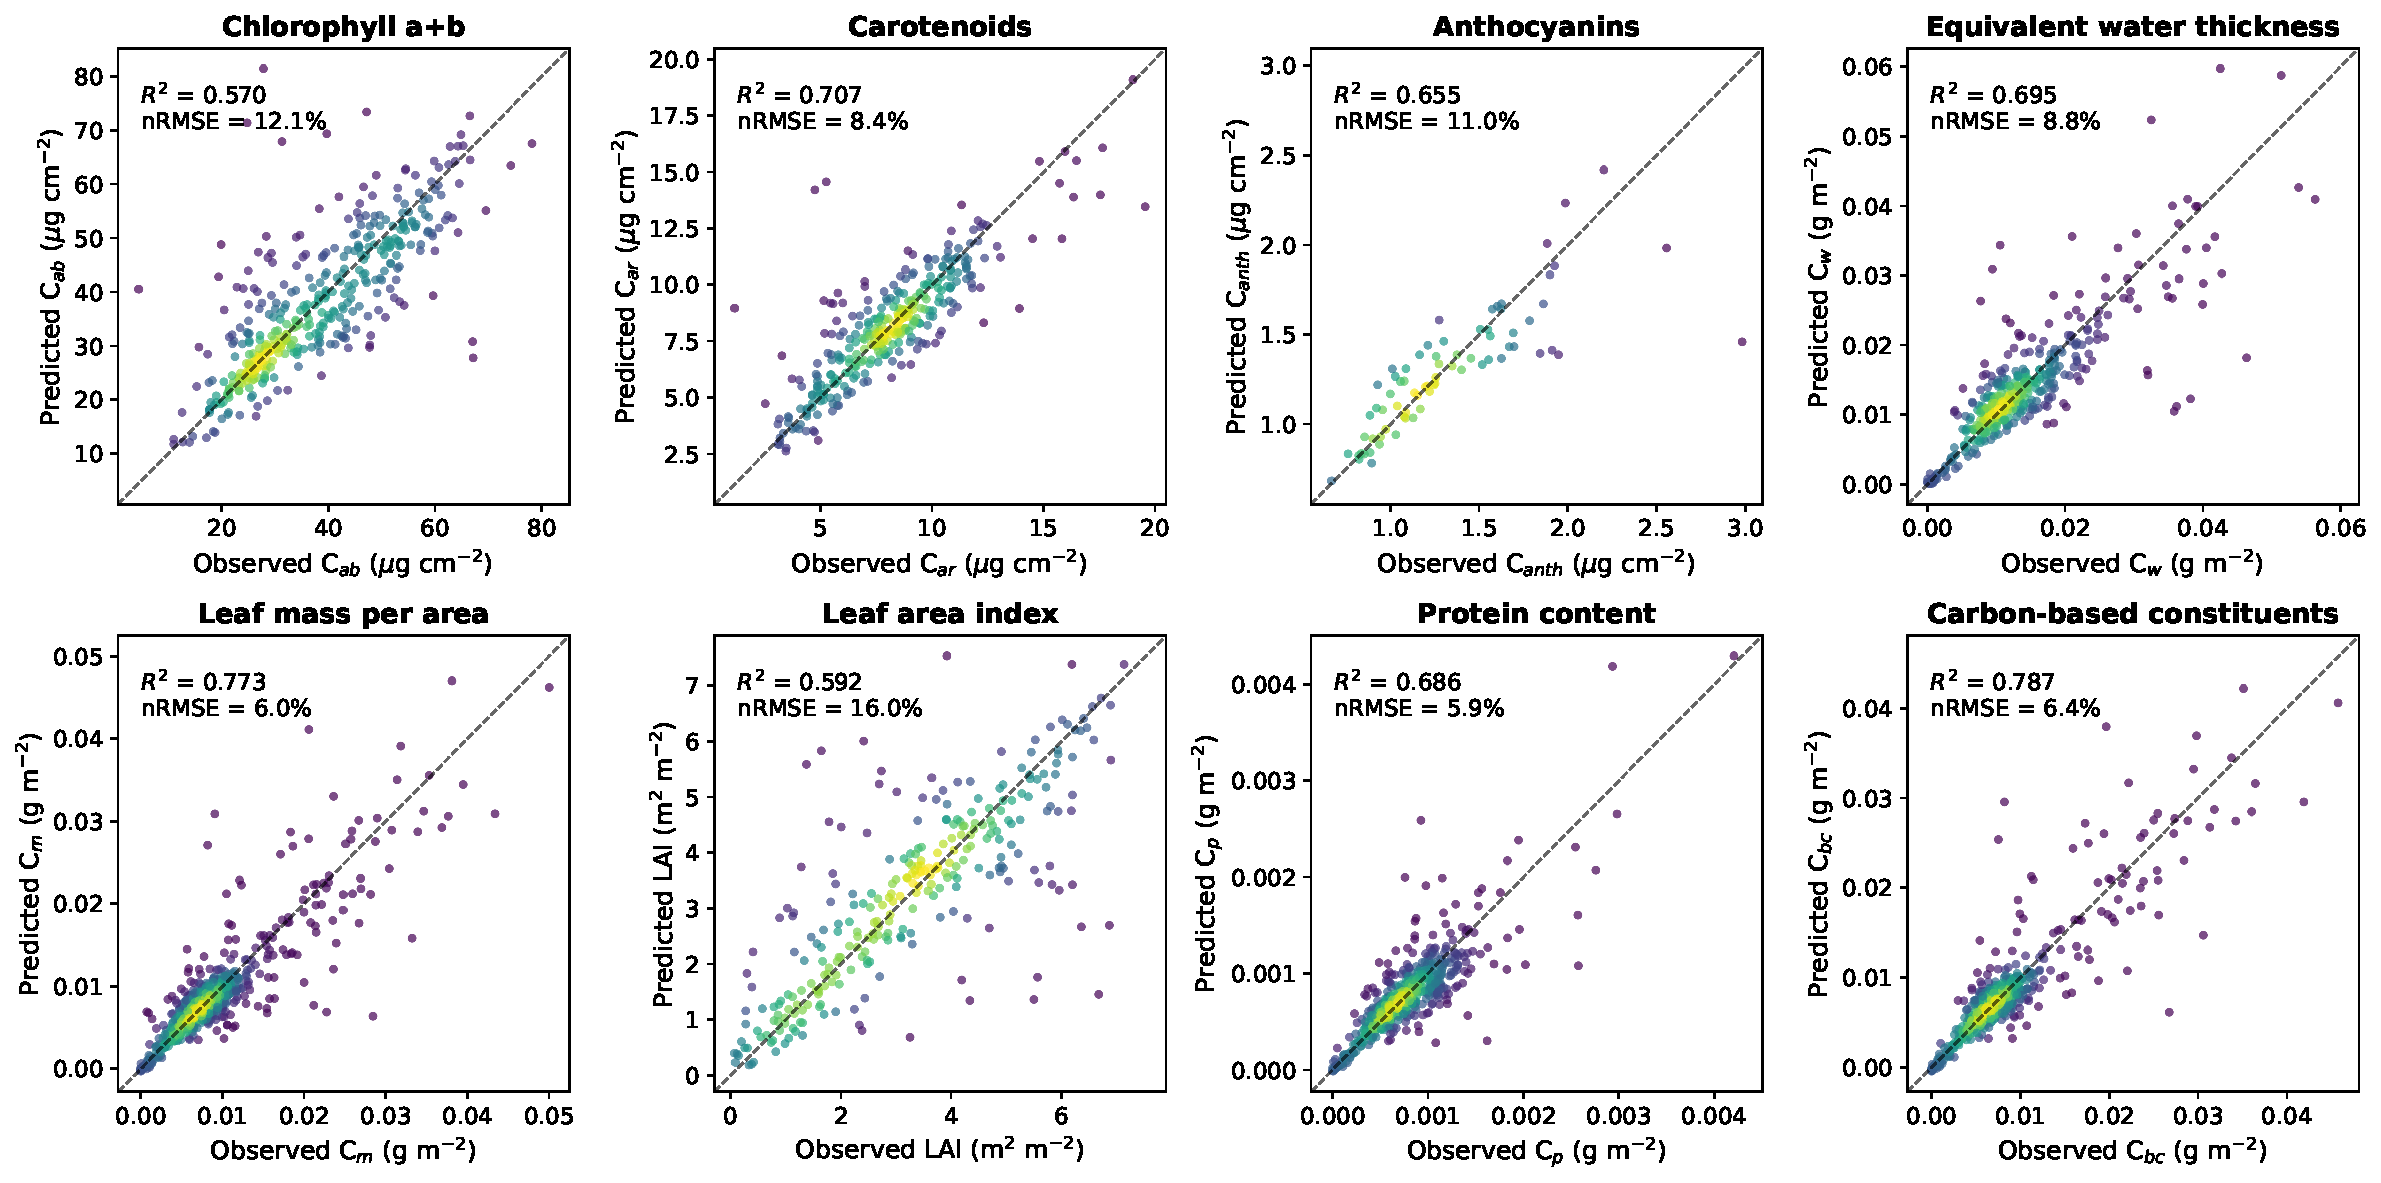
\includegraphics[width=\textwidth]{figures/scatterplot_best_model.pdf}
    \caption{Observed versus predicted trait values for the supervised 2D model (Reshape + EfficientNet-B0) on the GreenHyperSpectra test set ($n = 1{,}127$). Points are coloured by kernel density estimation. The dashed line represents the 1:1 relationship. $R^2$ and RMSE are reported for each trait. Not all test samples have measurements for every trait.}
    \label{fig:scatterplot}
\end{figure}

\subsection{Case Study 2: Self-Supervised Pretraining}
\label{sec:results_pretraining}

Table~\ref{tab:pretraining} compares the performance of supervised and self-supervised approaches across 1D and 2D representations. Among 1D methods reported by \citet{cherif2025greenhyperspectra}, the masked autoencoder with fine-tuning (MAE-1D FT) achieved the best performance ($R^2 = 0.645$), outperforming the supervised baseline by +0.058 and confirming the value of self-supervised pretraining on the 139,295 unlabeled spectra available in GreenHyperSpectra. The semi-supervised SR-GAN and physics-informed RTM-AE achieved only marginal improvements over the supervised baseline (+0.005 each).

Our 2D supervised approach (Reshape + EfficientNet-B0, $R^2 = 0.684 \pm 0.001$) surpassed all 1D methods, including the best self-supervised MAE-1D FT, by a margin of +0.039. This result demonstrates that the representational advantage conferred by 2D spectral images exceeds the benefit of self-supervised pretraining within the 1D framework. The MAE-2D with fine-tuning ($R^2 = 0.667 \pm 0.006$) also outperformed the 1D MAE-FT by +0.022, confirming that the 2D advantage extends to the self-supervised setting. However, the MAE-2D did not surpass the supervised 2D baseline, suggesting that with the current labeled dataset size ($n = 4{,}508$), the pretrained representations do not provide sufficient additional information beyond what direct supervised learning captures.

\begin{table}[htbp]
\centering
\caption{Comparison of pretraining strategies. All 2D methods use the Reshape transformation. Cherif baselines are from \citet{cherif2025greenhyperspectra}. Mean $R^2$ and standard deviation across three seeds are reported where available.}
\label{tab:pretraining}
\begin{tabular}{llcc}
\toprule
Method & Type & Mean $R^2$ $\pm$ std & $\Delta$ vs.\ Supervised 1D \\
\midrule
\multicolumn{4}{l}{\textit{Cherif et al.\ (2025) --- 1D baselines}} \\
Supervised EfficientNet-1D   & Supervised       & 0.587 $\pm$ 0.004 & -- \\
SR-GAN                        & Semi-supervised  & 0.592 $\pm$ 0.003 & +0.005 \\
RTM-AE                        & Physics-informed & 0.592 $\pm$ 0.004 & +0.005 \\
MAE-1D Linear Probing         & Self-supervised  & 0.604 $\pm$ 0.005 & +0.017 \\
MAE-1D Fine-Tuning            & Self-supervised  & 0.645 $\pm$ 0.003 & +0.058 \\
\midrule
\multicolumn{4}{l}{\textit{Ours --- 2D methods}} \\
\textbf{Supervised 2D (Reshape)} & Supervised    & \textbf{0.684 $\pm$ 0.001} & \textbf{+0.097} \\
MAE-2D Fine-Tuning            & Self-supervised  & 0.667 $\pm$ 0.006 & +0.080 \\
\bottomrule
\end{tabular}
\end{table}


The observation that supervised 2D training outperforms MAE-2D fine-tuning warrants further consideration. The MAE-2D encoder (ViT-Tiny, 2.8M parameters) is architecturally distinct from the supervised model (EfficientNet-B0, 4.0M parameters), and the gap may partly reflect the superior inductive biases of convolutional architectures for this image size and dataset scale. Additionally, the MAE pretraining converged rapidly (within approximately 10 epochs), with reconstruction loss approaching zero, suggesting that the 224$\times$224 Reshape images may not present sufficient reconstruction complexity to learn richly discriminative representations. Future work could explore larger encoder architectures, alternative masking strategies, or multi-scale patch sizes to improve the quality of pretrained features.
